\subsection{Wealth Formal Model} \label{wealth-formal-model}
Knowledge graphs follow Resource Description Framework (RDF)~\cite{w3crdf} as a means of data organization. Without loss of generality of how the form of the URIs is, data is stored in the form of triple \((s, p, o)\); a combination of a subject \(s\), a predicate \(p\), and an object \(o\) which can be visualized as nodes and directed-arc diagrams. For example, the statement "William Shakespeare's notable work is Romeo and Juliet" in human-readable URIs is mapped to the triple (\textit{WilliamShakespeare}, \textit{notableWork}, \textit{RomeoAndJuliet}). Likewise, the statement in Wikidata, which uses ID-based URIs, is mapped to (\textit{Q692}, \textit{P800}, \textit{Q83186}).

There are 3 kinds of nodes: IRIs, literals, and blank nodes. A triple is in the form of \((s, p, o) \in (I \cup B) \times I \times (I \cup B \cup L) \) where \(I\) is the node with type IRIs, \(B\) is the node with type of blank node, and \(L\) is the node with type of literals. In this study, we omit the usage of blank node, as this adds complexity to the analysis and may result in quality issue.

% \subsubsection{Class}
% In this study, we re-use the class model defined by Ramadizsa et al. (2023). A class is a group of entities that are the subject of the study. \textit{Human}, \textit{film}, and \textit{taxon} are some examples of class. In general, entity \(s\) is an instance of class \(C\) is expressed by the triple (\(s\), \textit{instanceOf}, \(C\)) or (\(s\), \textit{type}, \(C\)). We can get a more narrow class inside the defined class by specifying additional conditions, each consisting of a particular property and value associated with it. Example of such conditions for human class is \textit{gender} with associated value \textit{male}, while example for a country would be \textit{continent} with value \textit{Asia}. For instance, the class of human with gender male that lived during English Renaissance is queried using (\(?s\), \{(\(?s\), \textit{instanceOf}, \textit{human}), (\(?s\), \textit{gender}, \textit{male}), (\(?s\), \textit{timePeriod}, \textit{EnglishRenaissance})\}).

\subsubsection{Entity-Level Wealth: Knowledge Wealth Type and Definition}

Let \(s\) be any entity in a knowledge graph \(G\). We quantify the wealth of entity \(s\) in \(G\) as the amount of information about \(s\) available in \(G\). Thus, the knowledge wealth of an entity is defined by the number of properties associated/linked to it. For example, the wealth of William Shakespeare (Q692) in Wikidata counts all triples describing Q692 in Wikidata, including those detailing his family, occupation, image, and so on.

There are several notion on how to calculate the knowledge wealth of an entity: (1) wealth based on the (non-)uniqueness of individual property; (2) wealth based on type of property; and (3) wealth based on the direction of the link. The wealth of \(s\) with regard to graph \(G\) for each wealth category is denoted by \(W\), formalized and explained as follows.

\begin{figure}[!h]
    \centering
    \begin{subfigure}[b]{0.3\textwidth}
        \centering
        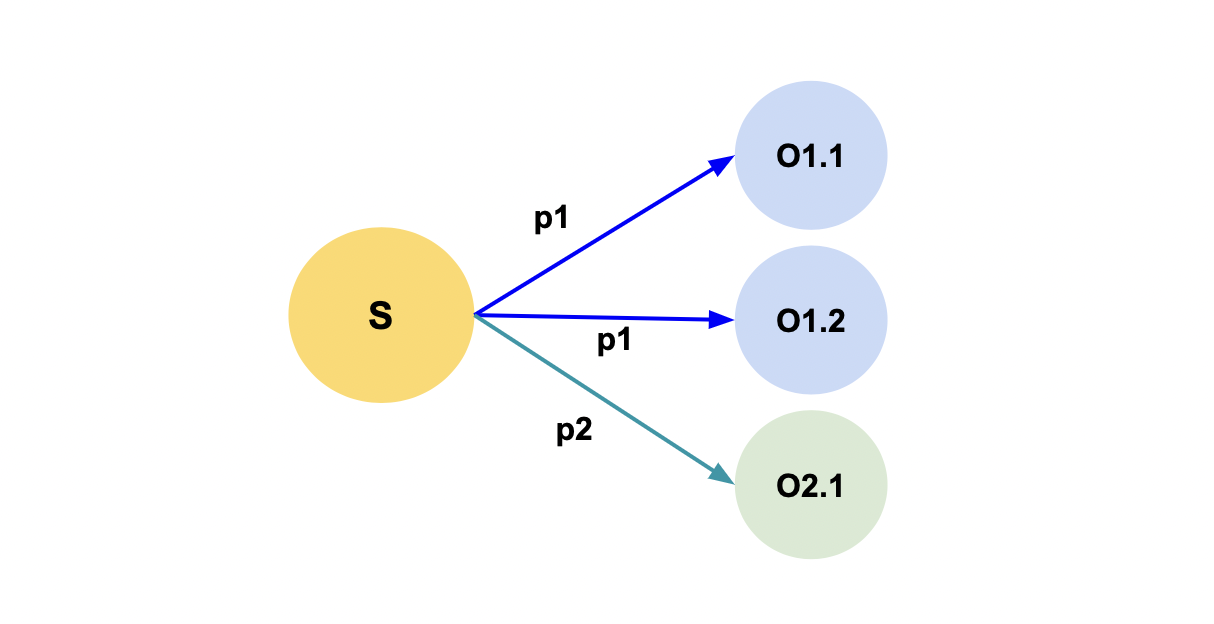
\includegraphics[scale=.3]{Wealth Type 1}
        \caption{Illustration of bag of properties and set of properties} \label{fig:wealth-type1}
    \end{subfigure}
    \hfill
    \begin{subfigure}[b]{0.3\textwidth}
        \centering
        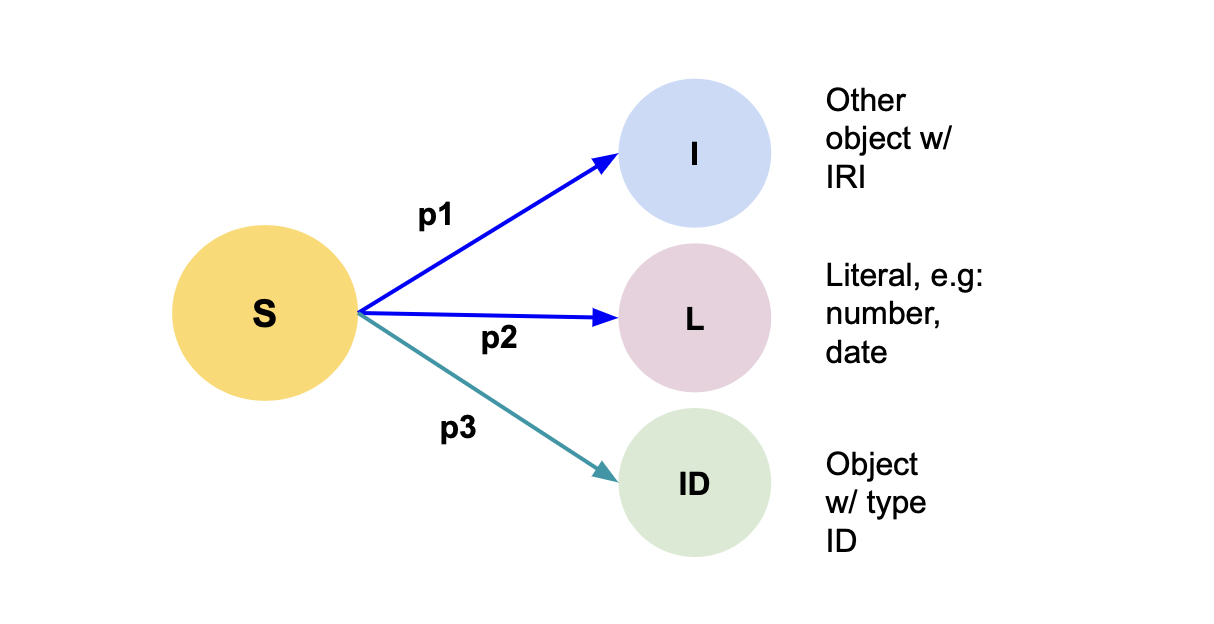
\includegraphics[scale=.3]{Wealth Type 2}
        \caption{Illustration of 3 types of property: object, literal, ID} \label{fig:wealth-type2}
    \end{subfigure}
    \hfill
    \begin{subfigure}[b]{0.3\textwidth}
        \centering
        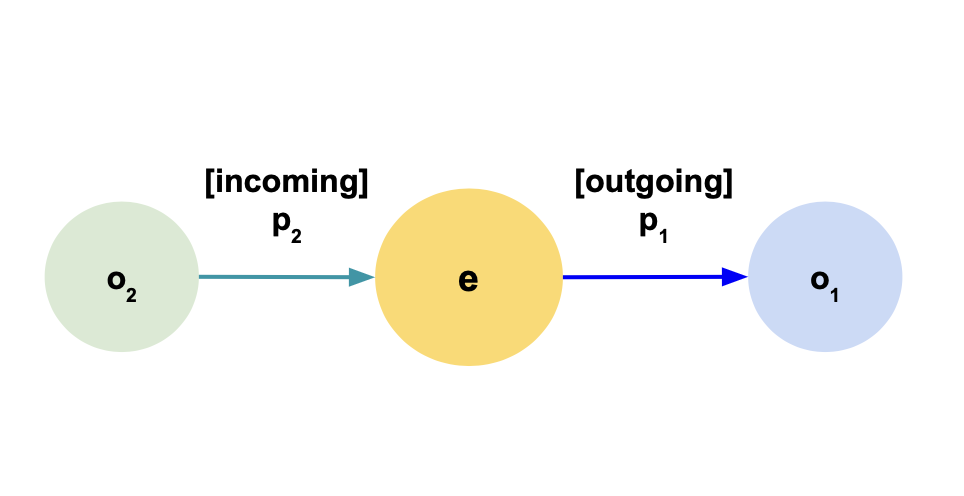
\includegraphics[scale=.3]{Wealth Type 3}
        \caption{Illustration of incoming link vs. outgoing link} \label{fig:wealth-type3}
    \end{subfigure}
    \caption{Three simple graphs} \label{fig:three graphs}
\end{figure}

\paragraph{Wealth based on the (non-)uniqueness of individual properties.}
The first measure of the knowledge wealth of \(s\) is bag of properties---the cardinality of set of all triples that has \(s\) in their subject position. In this definition, the triples \((s, p_1, o_1)\) and \((s, p_1, o_2)\) account for a wealth of 1 each, thus both have a total of 2.
Let \(N_{bag}(s,G)\) be a set that comprises all pair of predicate/property and object \((p,o)\) that is connected to \(s\). Then \(W_{bag}(s, G)\) is the cardinality of \(N_{bag}(s,G)\).
\[
    N_{bag}(s,G) = \{(p, o) | (s, p, o) \in G\}
\]
\[
    W_{bag}(s,G) = |N_{bag}(s)|
\]

Another way of measuring the wealth is by counting the number of distinct properties describing the entity, or set of properties. By this way, we are capturing the variety of information about an entity. In contrast to bag of properties, in set of properties \((s, p_1, o_1)\) and \((s, p_1, o_2)\) would be regarded as the "same" information because of the identical property \(p_1\), thus they only account for a total wealth of 1. Let \(N_{set}(s,G)\) be a set that comprises all predicate/property \(p\) that is connected to \(s\). Then \(W_{set}(s, G)\) is the cardinality of \(N_{set}(s,G)\).
\[
    N_{set}(s, G) = \{p | \exists o, (s, p, o) \in G\}
\]
\[
    W_{set}(s, G) = |N_{set}(s,G)|
\]

By the above definition, the wealth of entity \(s\) in \autoref{fig:wealth-type1} is 3 and 2, using bag of properties and set of properties respectively.

\paragraph{Wealth based on type of property.}
Object properties are other entities besides \(s\) that is connected with \(s\) through a property \(p\). Wealth of \(s\) using bag of properties with only considering the object properties is defined as:
\[
    W_{bag, object}(s, G) = |\{(p,o) | ((s, p, o) \in G) \cap (o \in I)\}|
\]
Literal properties are non-object properties that is connected with \(s\) through a property \(p\). Wealth of \(s\) using bag of properties with only considering the literal properties is defined as:
\[
    W_{bag, literal}(s, G) = |\{(p,o) | ((s, p, o) \in G) \cap (o \in L)\}|
\]

An external ID is a special type of string that is used to represent an entity in an external source. In Wikidata, an ID is identifiable by property type \textit{wikibase:ExternalId}. Just like any other property, an ID is connected with \(s\) through a property \(p\). Let  \(C_{ID,G}\) be a set comprising ID property in graph \(G\). Wealth of \(s\) using bag of properties with only considering the ID properties is defined as:
\[
    W_{bag, ID}(s, G) = |\{(p,o) | ((s, p, o) \in G) \cap (o \in L) \cap (o \in C_{ID,G})\}|
\]

\paragraph{Wealth based on the direction of the link.}
In outgoing link type of wealth, the properties that are used in the wealth calculation of an entity \(s\) are those obtained from link with outwards direction from that particular entity \(s\); that is where \(s\) appears to be the subject in the set of triples in graph \(G\). All types of wealth defined before use the notion of outgoing link.

In incoming link type of wealth, the properties that are used in the wealth calculation of an entity \(s\) are those obtained from link with inwards direction to that particular entity \(s\); that is where \(s\) appears to be the object in the set of triples in graph \(G\). To illustrate, let \(N_{bag}(s)\) be a set that comprises all pair of object and predicate/property \((o,p)\) that is connected to \(s\) in incoming direction to \(s\) i.e., \(N_{bag}(s)\) = \(\{(o, p) | (o, p, s) \in G\}\). Then the wealth of \(s\) using bag of properties and the view of incoming link is notated as \(W_{bag, incoming}(s, G)\), and equal to the cardinality of \(N_{bag}(s)\).
\[
    N_{bag, incoming}(s, G) = \{(o,p) | (o, p, s) \in G\}
\]
\[
    W_{bag, incoming}(s, G) = |N_{bag, incoming}(s, G)|
\]

Looking at in \autoref{fig:wealth-type3}, the wealth of entity \(s\) is 1 using outgoing link, which is from the triple \((s, p_1, o1)\). Its wealth is also 1 and using incoming link, which comes from the triple \((o2, p_2, s)\).

Each definition above can be used simultaneously. For example, the wealth of entity \(s\) using set of properties, calculating object and data but not ID properties, and using the direction of outgoing link is denoted by \(W_{set, outgoing, (object \cup data) \cap ID^\complement}(s, G) = |N_{set, outgoing, (object \cup data) \cap ID^\complement}(s, G)|\) with \(N_{set, outgoing, (object \cup data) \cap ID^\complement}(s, G) = \{p | \exists o, (s, p, o) \in G, \cap (o \in ((I \cup L) \cap C_{ID,G}^\complement)\}\)

\subsubsection{Class-Level Wealth}
In this study, we re-use the class model defined by Ramadizsa et al.~\cite{RamadizsaDNR23}. A class is a group of entities that are the subject of the study. \textit{Human}, \textit{film}, and \textit{taxon} are some examples of class. In general, entity \(s\) is an instance of class \(C\) is expressed by the triple (\(s\), \textit{instanceOf}, \(C\)) or (\(s\), \textit{type}, \(C\)). We can get a more narrow class inside the defined class by specifying additional conditions, each consisting of a particular property and value associated with it. Example of such conditions for human class is \textit{gender} with associated value \textit{male}, while example for a country would be \textit{continent} with value \textit{Asia}. For instance, the class of human with gender male that lived during English Renaissance is queried using (\(?s\), \{(\(?s\), \textit{instanceOf}, \textit{human}), (\(?s\), \textit{gender}, \textit{male}), (\(?s\), \textit{timePeriod}, \textit{EnglishRenaissance})\}).

Let \(C\) be a class that consists of \(m\) distinct entities \(s_1\), \(s_2\), ... \(s_m\) in graph \(G\). We define \(T_C\) a multiset consisted of the wealth of each entity of \(C\), i.e., \[T_C = \{W(s_1), W(s_2), W(s_3), ..., W(s_m)\}.\] The overall wealth of class \(C\) can be be quantified using its constituent entities and be expressed as a function of \(T_C\), denoted as \(f(T_C)\), where \(f\) may represent statistical summaries such as the cardinality (i.e., entity count), mean, median, mode, or percentile of its entities's wealth. For example, let a class \(C\) consists of 4 entities  \(s_1\), \(s_2\), \(s_3\), and \(s_4\) from \autoref{fig:wealth-weighted}. If we use cardinality as the function \(f\), then the wealth of class \(C\) is 4, corresponding to the number of entities it contains.